\documentclass[tikz,border=3pt]{standalone}
\usetikzlibrary{arrows.meta}
\begin{document}
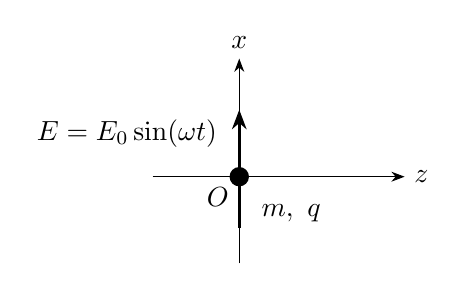
\begin{tikzpicture}[scale=1.0,>=Stealth,line width=0.9pt]
  % 座標軸
  \draw[line width=0.4pt,->] (-1.1,0) -- (2.1,0) node[right] {$z$};
  \draw[line width=0.4pt,->] (0,-1.1) -- (0,1.5) node[above] {$x$};
  \node[below left] at (0,0) {$O$};

  % 荷電粒子 (m, q)
  \fill (0,0) circle (3.5pt);
  \node[below right,yshift=-2pt] at (0.15,-0.15) {$m,\ q$};

  % 入射電磁波の電場成分の矢印（x方向）
  \draw[->] (0,-0.65) -- (0,0.85);
  \node[left] at (-0.15,0.55) {$E = E_0\sin(\omega t)$};
\end{tikzpicture}
\end{document}
